\documentclass{template/openetcs_report}
% Use the option "nocc" if the document is not licensed under Creative Commons
%\documentclass[nocc]{template/openetcs_article}
\usepackage{lipsum,url}
\usepackage{supertabular}
\usepackage{multirow}
\usepackage{color, colortbl}
\usepackage{hyperref}
\usepackage{listings}
\usepackage{makeidx}
\definecolor{gray}{rgb}{0.8,0.8,0.8}
\usepackage[modulo]{lineno}
\usepackage{float}
\usepackage{fixme}
\usepackage{pdflscape}
\usepackage[acronym, % list of acronyms
  %section, % add the glossary to the table of content
            %description,% acronyms have a user-supplied description,
 style=longheader, % table style
 nonumberlist % no page number
  ]{glossaries}

\graphicspath{{./template/}{.}{./images/}}

\renewcommand*{\glspostdescription}{} %Deactivate point at the end of every description
\renewcommand*{\glossaryname}{Glossary}

%create glossary
% \makeglossaries
 %Glossary terms
% \loadglsentries{glossary}

\begin{document}
\frontmatter
\project{openETCS}

\newcommand{\define}[1]{\index{#1}\emph{#1}}



%Please do not change anything above this line
%============================

% The document metadata is defined below

%assign a report number here
\reportnum{OETCS/WP3/D3.5.2}

%define your workpackage here
\wp{Work Package 3: ``Modeling''}

%set a title here
\title{openETCS Design Specification}

%set the date of the report here
\date{May 2015}


%document approval
%define the name and affiliation of the people involved in the documents approbation here
\creatorname{Baseliyos Jacob}
\creatoraffil{DB Netz AG}

\techassessorname{Jan Welte}
\techassessoraffil{Technische Universität Braunschweig}

\qualityassessorname{Izaskun de la Torre}
\qualityassessoraffil{SQS}

\approvalname{Klaus-R\"udiger Hase}
\approvalaffil{DB Netz}


%define a list of authors and their affiliation here

\author{Baseliyos Jacob, Peter Mahlmann}
\affiliation{DB Netz AG}




% define the coverart
\coverart[width=350pt]{openETCS_EUPL}

\newpage
%define the type of report
\reporttype{Architecture and Design Specification}


\begin{abstract}
%define an abstract here
This document gives an introduction to the software and component design of the openETCS OBU model. The functional scope is tailored to cover the functionality required for the openETCS demonstration as an objective of the ITEA2 project. The goal is to develop a formal model and to demonstrate the functionality during a proof of concept on the ETCS Level 2 Utrecht Amsterdam track with real scenarios. It has to be read as a complement to the models in SysML and Scade languages. 
\end{abstract}

%=============================
\maketitle

%Modification history
%if you do not need a modification history table for your document simply comment out the eight lines below
%=============================


\chapter*{Modification History}
\tablefirsthead{
\hline 
\rowcolor{gray} 
Version & Section & Modification / Description & Author & Date \\\hline}
\begin{supertabular}{| m{1.2cm} | m{1.5cm} | m{4.0cm} | m{3.5cm} | m{3.5cm} |}
0.1 & Document & Initial document providing structure & Peter Mahlmann& 27.05.2015 \\\hline
\end{supertabular}

% list subsubsections in table of contents
\setcounter{tocdepth}{3}


\tableofcontents
\listoffiguresandtables
\newpage
%=============================

%Uncomment the next line if you need line numbers for tracebility when the document is in review
%\linenumbers
%=============================


% The actual document starts below this line
%=============================

\mainmatter


\chapter{Runtime API}

\section{Introduction to the Architecture}

\subsection{Abstract Hardware Architecture}

For proper understanding of openETCS API and of constraints imposed on
both sides of the API, we need to define a \emph{reference abstract hardware architecture}. This hardware architecture is ``abstract''
is the sense that the actual vendor specific hardware architecture
might be totally different of the abstract architecture described in
this chapter. For example, several units might be grouped together on
the same processor.

However, the actual vendor specific architecture shall fulfill all the
requirements and constraints of this reference abstract hardware
architecture and shall not request additional constraints.

\subsection{Definition of the Reference Abstract Hardware Architecture}

\begin{figure}
  \centering
  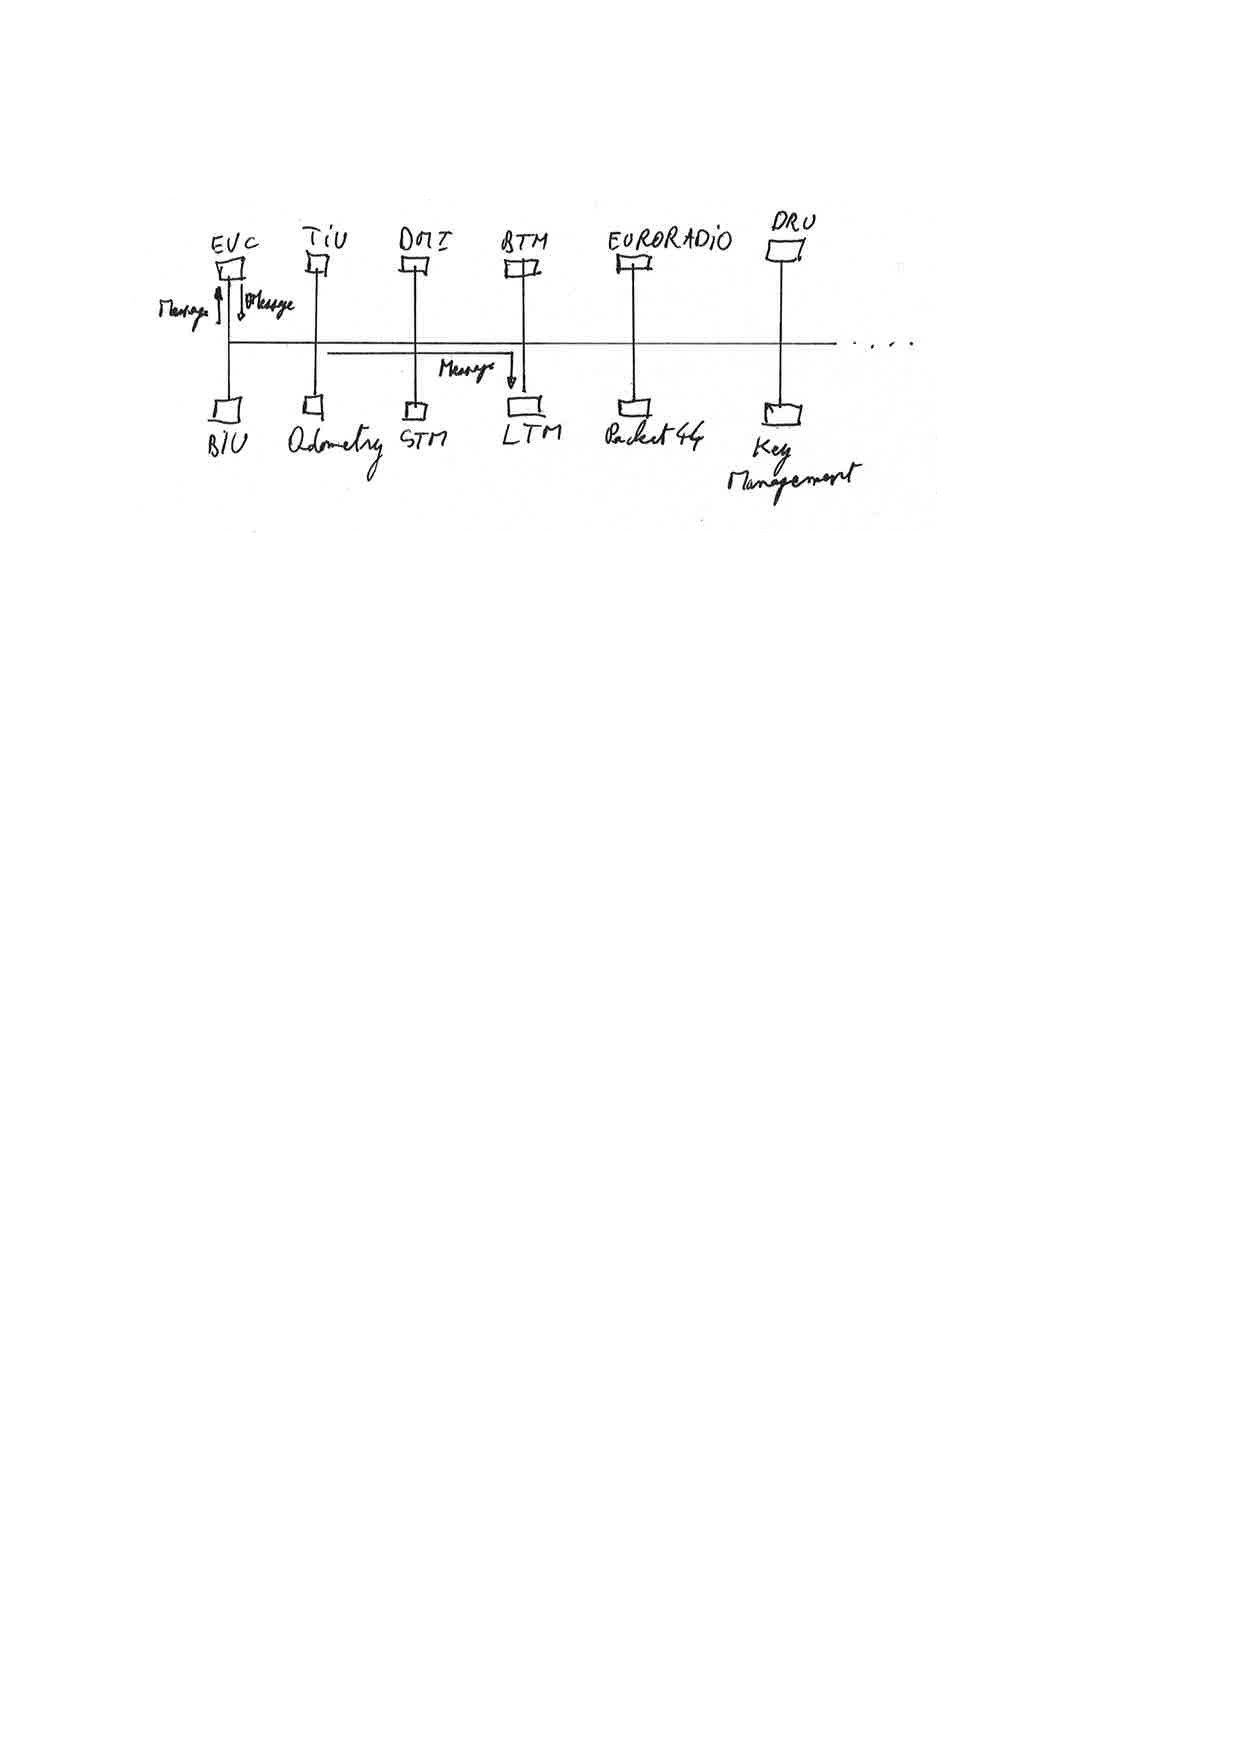
\includegraphics[width=\textwidth]{abstract-hardware-architecture.pdf}
  \caption{Reference abstract hardware architecture.}
  \label{fig:hardware-arch}
\end{figure}

The reference abstract hardware architecture is shown in Figure
\ref{fig:hardware-arch}. The reference abstract hardware architecture is made of a bus on which are connected \emph{units} defining the OBU:

\begin{itemize}
\item {EVC};
\item {TIU};
\item {ODO};
\item {DMI};
\item {STM};
\item {BTM};
\item {LTM}: Not part of this openETCS implementation;
\item EURORADIO;
\item {JRU}: Not part of this openETCS implementation;
\end{itemize}

Elements not being part of this implementation are marked. Those units shall working concurrently. They shall exchange information with other units through asynchronous message passing.

\subsection{Reference abstract software architecture}
\label{software-arch}

\begin{figure}
  \centering
  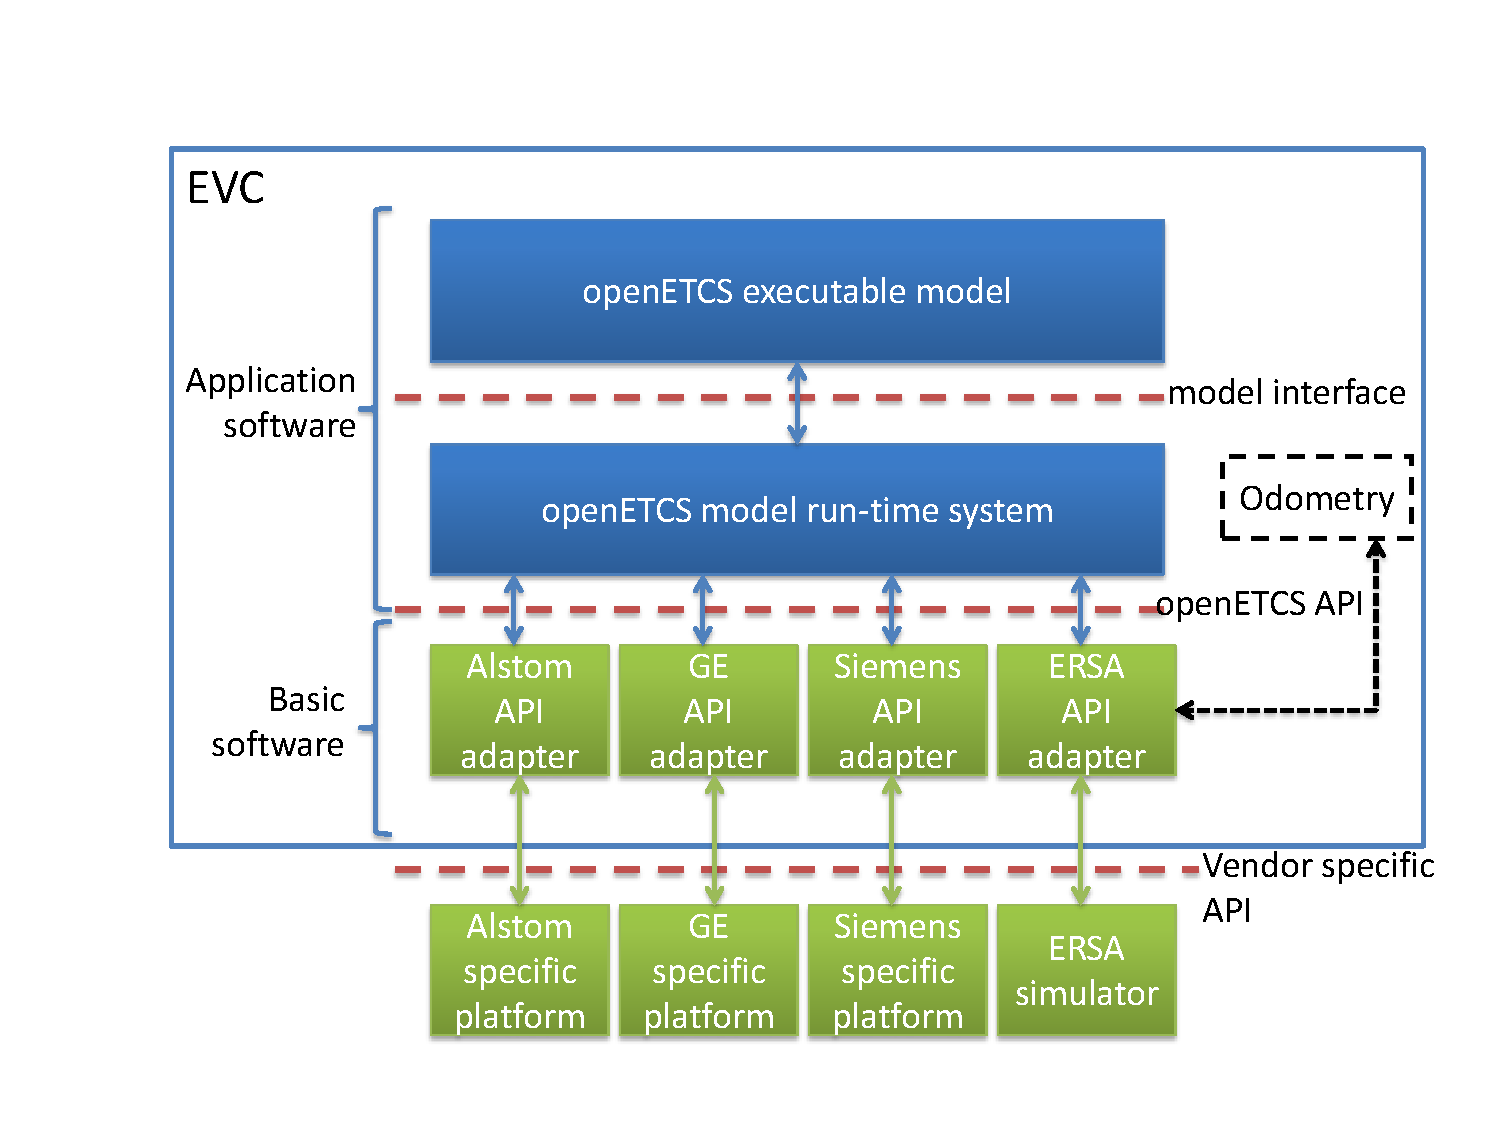
\includegraphics[width=0.9\textwidth]{software-architecture.pdf}
  \caption{Reference abstract software architecture}
  \label{fig:software-arch}
\end{figure}

The \emph{reference abstract software architecture} is shown in Figure
\ref{fig:software-arch}. This architecture consists of following
elements:
\begin{description}
\item[openETCS executable model] produced by the SCADE model \cite{scade-model}. It shall contain the program implementing core
  ETCS functions;
\item[openETCS model run-time system] shall help the execution
  of the openETCS executable model by providing additional functions
  like encode/decode messages, proper execution of the model through
  appropriate scheduling, re-order or prioritize messages, etc. 
\item[Vendor specific API adapter] shall make the link between
  the Vendor specific platform and the openETCS model run-time system.
  It can buffer message parts, encode/decode messages, route messages
  to other EVC components, etc.
\item[EVC] All above three elements shall be included in the EVC;
\item[Vendor specific platform] shall be all other elements of
  the system, bus and other units, as shown in Figure \ref{fig:hardware-arch}.
\end{description}

We have thus three interfaces:
\begin{description}
\item[Model interface]
 is the interface between openETCS executable model and openETCS model run-time system. 
\item[openETCS {API}]
 is the interface between openETCS model run-time system and Vendor specific {API} adapter.
\item[Vendor specific {API}]
 is the interface between Vendor specific {API} adapter and Vendor specific platform. This interface is not publicly described for all vendors. You can find the Alstom implementation as an example.
\end{description}

The two blocks openETCS executable model and openETCS model run-time
system are making the \emph{application software} part. This application software might be either openETCS reference software or vendor specific software.

The Vendor specific API adapter is making the \emph{Basic software} part.







\bibliographystyle{unsrt}
\bibliography{architecture}


\addcontentsline{toc}{chapter}{Index}
\printindex
%===================================================
%Do NOT change anything below this line

\end{document}
